\chapter{Estado del Arte}
\label{ch:state_of_the_art}

\section{Contexto histórico y arquitectura del sistema de distribución eléctrica}
\label{sec:contexto_historico_arquitectura}

Antes de abordar en detalle la problemática técnica del concentrador de datos de nueva generación, resulta conveniente situar el problema dentro de su contexto histórico y sistémico. Por un lado, las comunicaciones por línea eléctrica (\textit{Power Line Communications, PLC}) no constituyen una tecnología emergente, sino la evolución de más de un siglo de soluciones de telecontrol sobre la propia red de distribución. Por otro lado, el propio concentrador solo se entiende como pieza de un sistema eléctrico más amplio, con una cadena de valor, unos agentes regulados y una infraestructura física (los centros de transformación) sobre la que se apoya toda la telegestión moderna. Las siguientes secciones recorren brevemente ambos aspectos antes de profundizar en la arquitectura específica de los centros de transformación inteligentes.

\subsection{Evolución histórica de las comunicaciones por línea eléctrica (PLC)}
\label{subsec:evolucion_plc}

El uso de la propia red eléctrica como medio de transmisión de información es casi tan antiguo como la propia red de distribución. Ya en la década de 1920 se documentan los primeros sistemas de telemetría sobre líneas de alta tensión, operando en el rango de 15 a 500 kHz \cite{SHARMA2017704}. Luego, en torno a 1930, aparecieron los primeros sistemas de comunicación de banda ultraestrecha (\textit{Ultra-Narrowband PLC, UNB-PLC}), como el sistema TWACS (\textit{Two-Way Automatic Communication System}), concebido para operar de forma óptima sobre la frecuencia fundamental de 60 Hz de la propia red de transporte y distribución \cite{SHARMA2017704}. Estos antecedentes evidencian que la idea de emplear el cableado eléctrico como canal de comunicación es, en esencia, tan antigua como la propia electrificación masiva.

\begin{figure}[ht]
    \centering
    % 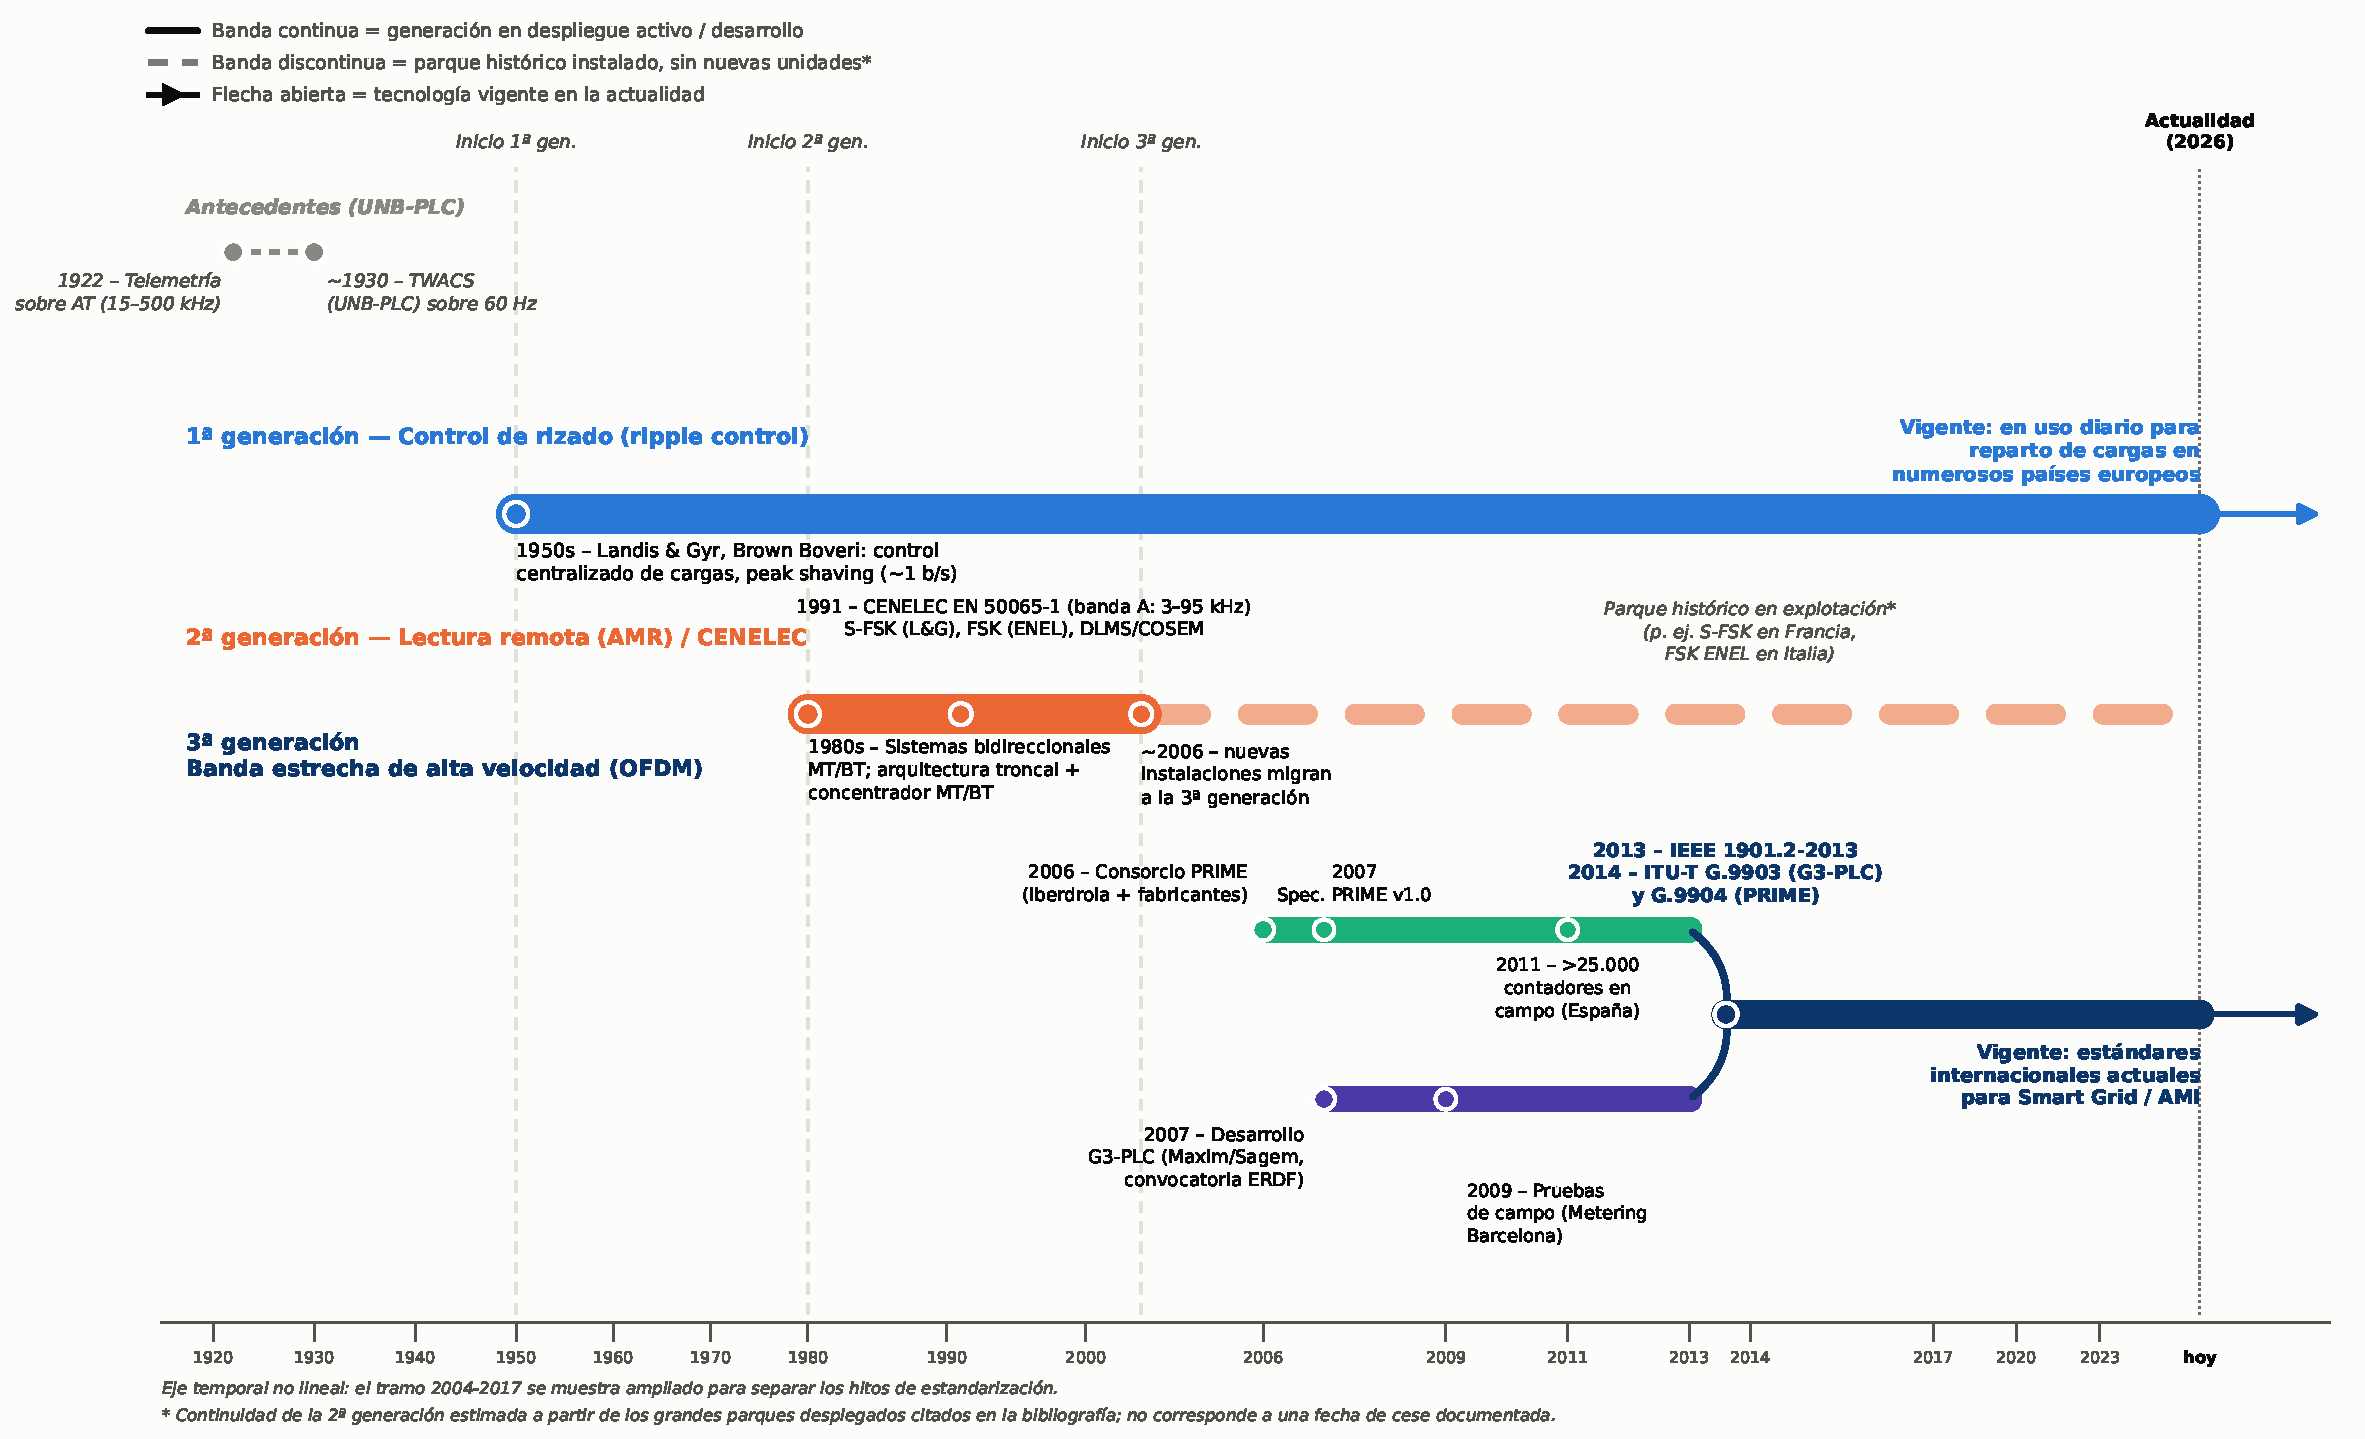
\includegraphics[width=\textwidth]{Imagenes/linea_tiempo_evolucion_PLC.pdf}
    \caption{Línea temporal de la evolución histórica de las comunicaciones PLC aplicadas a la red eléctrica, desde el control de rizado hasta los estándares OFDM de banda estrecha actuales.}
    \label{fig:linea_tiempo_plc}
\end{figure}

\subsubsection{Primera generación: el control de rizado (\textit{ripple control})}
\label{subsubsec:ripple_control}

La primera generación de comunicaciones PLC con vocación de control masivo sobre la red de distribución surge en la década de 1950, de la mano de fabricantes como Landis \& Gyr o Brown Boveri, quienes desarrollaron los sistemas de \textbf{control de rizado} (\textit{ripple control}) para la gestión centralizada de cargas y el achatamiento de picos de demanda (\textit{peak shaving}) \cite{5764444}. Estos sistemas, todavía en uso en numerosos países europeos, inyectan una señal de audiofrecuencia (típicamente entre 150 y 1350 Hz, evitando los armónicos de 50/60 Hz) en la red de media tensión (MT), con niveles de potencia de hasta 150 kVA que permiten que la señal atraviese con facilidad los transformadores MT/BT y alcance de forma simultánea a todos los receptores conectados a una amplia área de baja tensión (BT) \cite{5764444}.

Se trata, no obstante, de una comunicación unidireccional y de muy baja tasa de datos (del orden de 1 bit por segundo), suficiente para transmitir órdenes de conmutación de relés (encendido o apagado de calefactores, termos eléctricos o alumbrado público) o para señalizar los cambios de tarifa horaria a los contadores electromecánicos, pero completamente inadecuada para aplicaciones bidireccionales como la lectura remota de contadores \cite{5764444}.

\subsubsection{Segunda generación: lectura remota de contadores y normalización CENELEC}
\label{subsubsec:segunda_generacion_amr}

La necesidad de aplicaciones de \textbf{Automatización de la Distribución} (\textit{Distribution Automation, DA}) y de \textbf{Lectura Automática de Contadores} (\textit{Automatic Meter Reading, AMR}) con comunicación bidireccional impulsó, a partir de la década de 1980, el desarrollo de una segunda generación de sistemas PLC de mayor frecuencia portadora y, por tanto, de menor alcance a través de los transformadores MT/BT \cite{5764444}. Esta limitación de propagación obligó a introducir por primera vez una arquitectura jerárquica de dos niveles: una red troncal en MT y, en cada centro de transformación, una pasarela o concentrador que distribuye las comunicaciones en BT hasta el usuario final, arquitectura que en esencia se mantiene vigente en los concentradores de datos actuales \cite{5764444}.

En 1991, el comité europeo de normalización electrotécnica CENELEC publicó la norma EN 50065-1, que reserva la banda de 3 a 95 kHz (\textbf{banda CENELEC-A}) en exclusiva a las compañías distribuidoras de energía y sus licenciatarios para aplicaciones de telegestión y automatización de red, dejando las sub-bandas B, C y D (hasta 148,5 kHz) para aplicaciones del usuario final \cite{EN50065_1, 5764444}. Bajo este marco normativo proliferaron soluciones propietarias de baja velocidad, como el sistema S-FSK de Landis \& Gyr, ampliamente desplegado en Francia, o el sistema FSK de ENEL, que en Italia llegó a cubrir más de 30 millones de contadores \cite{5764444}. En esta misma etapa surge además la pila de aplicación DLMS/COSEM, que independiza el modelo de datos de facturación y medida del protocolo de comunicación subyacente (PLC, módem telefónico o red celular), y que continúa siendo la base de la telemedida moderna \cite{5764444}.

\subsubsection{Tercera generación: banda estrecha de alta velocidad y la aparición de PRIME}
\label{subsubsec:tercera_generacion_ofdm}

Las exigencias de las aplicaciones de automatización en tiempo real y de gestión avanzada de medida (\textit{Advanced Metering Management}) superaron pronto las tasas de transmisión de la segunda generación. La respuesta tecnológica llegó de la mano de la modulación multiportadora (\textit{Orthogonal Frequency Division Multiplexing, OFDM}), ya consolidada en otros ámbitos de las telecomunicaciones (xDSL, TV digital terrestre, redes celulares 3G), y cuya robustez frente a canales selectivos en frecuencia la hace especialmente adecuada para el hostil canal eléctrico \cite{5764444}.

De forma resumida, y sin ánimo de profundizar en ello puesto que no es el objeto de este trabajo, la modulación OFDM divide el ancho de banda disponible en un elevado número de subportadoras ortogonales de banda muy estrecha, en lugar de emplear una única portadora de banda ancha como hacían los sistemas FSK o S-FSK de la generación anterior. Al ser tan estrecho el intervalo de frecuencia que ocupa cada subportadora, el canal se percibe de forma prácticamente plana dentro de dicho intervalo, aun cuando la respuesta global del canal eléctrico sea marcadamente selectiva en frecuencia. Además, la inserción de un intervalo de guarda (prefijo cíclico) entre símbolos absorbe la dispersión temporal provocada por las reflexiones y discontinuidades de impedancia propias de la red eléctrica, evitando la interferencia entre símbolos y permitiendo una ecualización muy sencilla en el receptor. Esta capacidad de descomponer un canal hostil y distorsionado en múltiples subcanales casi ideales es precisamente lo que hace a OFDM mucho más robusto frente al ruido de banda estrecha, las muescas de atenuación (\textit{notches}) y las interferencias impulsivas del canal PLC, y explica por qué se convirtió en la elección natural para las nuevas generaciones de estándares de banda estrecha de alta velocidad \cite{5764444}.

Sobre esta base nace en 2006 el consorcio impulsor del estándar \textbf{PRIME} (\textit{PoweRline Intelligent Metering Evolution}), formado inicialmente por Iberdrola junto a fabricantes de contadores y semiconductores, cuya primera especificación se publica en 2007 \cite{5764444, SHARMA2017704}. En paralelo, a raíz de una convocatoria de ERDF (Francia), surge el estándar competidor \textbf{G3-PLC}, y ambas familias tecnológicas terminan por converger en los estándares internacionales \textbf{IEEE 1901.2-2013} e \textbf{ITU-T G.9904/G.9903} \cite{SHARMA2017704, 5764444}. Iniciativas europeas como el proyecto \textbf{DLC+VIT4IP}, financiado por el 7º Programa Marco de la Comisión Europea, extendieron además estas tecnologías hacia el uso del protocolo IPv6 y bandas de hasta 500 kHz, sentando las bases de la arquitectura de comunicaciones que emplean los concentradores de datos de última generación \cite{5764443}. Esta tercera generación es, precisamente, el punto de partida tecnológico sobre el que se construyen los desarrollos descritos en el resto de este capítulo.

\subsection{De la generación al usuario: la cadena de valor del sistema eléctrico}
\label{subsec:cadena_valor_electrico}

De forma anecdótica, resulta útil recordar el recorrido físico que realiza la electricidad hasta llegar a una vivienda, puesto que sobre ese mismo recorrido se apoya toda la infraestructura de comunicaciones descrita en este trabajo. La energía se genera en centrales de distinta naturaleza (nucleares, de ciclo combinado, eólicas, fotovoltaicas, hidroeléctricas, etc.) a tensiones relativamente bajas, que se elevan mediante transformadores hasta niveles de \textbf{alta tensión} (AT, típicamente 132 a 400 kV) para minimizar las pérdidas óhmicas durante el transporte a larga distancia a través de la red de transporte. En las proximidades de los núcleos de consumo, subestaciones transformadoras reducen esta tensión a niveles de MT (habitualmente 15 o 20 kV en España), que discurre por la red de distribución urbana o rural hasta alcanzar, finalmente, los \textbf{centros de transformación} (CT) de MT/BT, donde se reduce por última vez la tensión hasta los 400/230 V de la red de BT que llega ya, a través de la acometida, a cada vivienda o local.

\begin{figure}[ht]
    \centering
    % 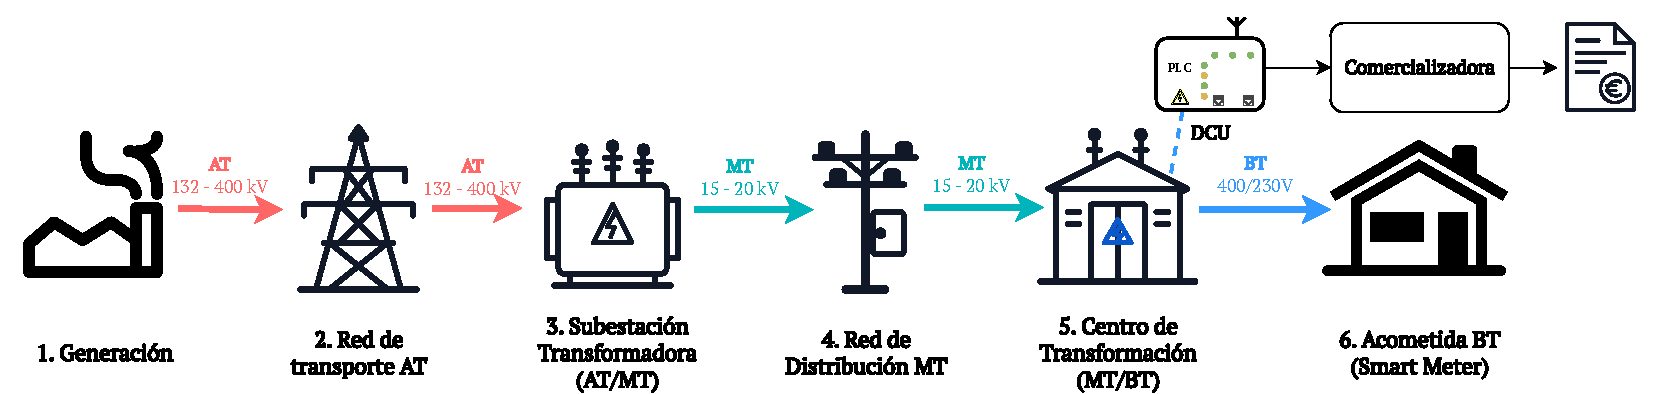
\includegraphics[width=\textwidth]{Imagenes/cadena_valor_sistema_electrico.pdf}
    \caption{Cadena de valor del sistema eléctrico, desde la generación hasta el punto de consumo, pasando por el transporte, la distribución y los centros de transformación MT/BT.}
    \label{fig:cadena_valor_electrico}
\end{figure}

\subsubsection{Distribuidoras y comercializadoras: el mercado eléctrico liberalizado}
\label{subsubsec:distribuidora_comercializadora}

Conviene distinguir, dentro de esta cadena, dos figuras que con frecuencia se confunden desde la perspectiva del usuario final. La \textbf{distribuidora} es la empresa regulada, en régimen de monopolio natural en su zona de concesión, propietaria y responsable del mantenimiento de la red física de MT y BT, de los CTs y de los propios equipos de medida instalados en los domicilios de los usuarios. La \textbf{comercializadora}, por su parte, es el agente que opera en régimen de libre competencia dentro del mercado liberalizado, adquiriendo energía en el mercado mayorista y facturándola al cliente final, sin ser propietaria de ningún activo físico de la red. Esta separación de actividades (conocida como \textit{unbundling}), habitual en la literatura anglosajona bajo la denominación (\textit{Distribution System Operator, DSO}) para referirse a la distribuidora \cite{5764443}, implica una consecuencia relevante para este trabajo: aunque el usuario reciba su factura de una comercializadora, el contador y toda la cadena de telemedida (contador, red PLC, concentrador y sistemas centrales) pertenecen y son operados por la distribuidora, que es quien recibe en última instancia los datos de consumo recopilados por el concentrador de datos.

\subsection{Los centros de transformación MT/BT: estructura y esquemas constructivos}
\label{subsec:estructura_ct}

El CT es la instalación eléctrica encargada de reducir la tensión de MT a BT y de repartir esta última entre los distintos circuitos de la red de baja tensión que alimentan a los usuarios finales de una determinada área geográfica. Con independencia de su ubicación, todo CT comparte una estructura eléctrica similar, compuesta esencialmente por: celdas de línea de entrada y salida en MT, que permiten conectar el centro en anillo o en derivación a la red de distribución; una celda de protección (interruptor-fusible combinado o interruptor automático) que protege al transformador frente a sobrecargas y cortocircuitos; el propio transformador de potencia MT/BT; y un cuadro de baja tensión desde el que parten los distintos circuitos o salidas de la red de BT, habitualmente organizados en esquema radial o en anillo abierto hacia las acometidas de los usuarios.

Constructivamente, sin embargo, los CT adoptan tipologías muy diversas en función del entorno urbano o rural en el que se instalan:
\begin{itemize}
    \item \textbf{CT de interior o en edificio:} integrado dentro de un local en la planta baja o el subsuelo de una edificación, es la solución habitual en entornos urbanos densos.
    \item \textbf{CT prefabricado tipo caseta:} una envolvente de hormigón u obra civil prefabricada, autoportante, que se instala directamente sobre el terreno y que constituye la solución más extendida en urbanizaciones y polígonos industriales.
    \item \textbf{CT subterráneo:} instalado bajo la vía pública, en una arqueta o bóveda enterrada, minimizando el impacto visual y el uso de suelo en centros urbanos con alta densidad de carga.
    \item \textbf{CT de intemperie o sobre poste (aéreo):} el transformador se instala directamente sobre un apoyo de la red aérea de MT, siendo la solución más económica y habitual en entornos rurales de baja densidad de carga.
\end{itemize}

\begin{figure}[ht]
    \centering
    % \includegraphics[width=0.85\textwidth]{Imagenes/tipos_constructivos_CT.pdf}
    \caption{Tipologías constructivas más habituales de los centros de transformación MT/BT: interior, prefabricado tipo caseta, subterráneo e intemperie sobre poste.}
    \label{fig:tipos_ct}
\end{figure}

\begin{figure}[ht]
    \centering
    % \includegraphics[width=0.85\textwidth]{Imagenes/esquema_unifilar_CT.pdf}
    \caption{Esquema unifilar simplificado de un centro de transformación MT/BT, con celdas de línea de entrada/salida en anillo, celda de protección del transformador y cuadro de baja tensión.}
    \label{fig:esquema_unifilar_ct}
\end{figure}

Es precisamente sobre esta infraestructura, común a decenas de miles de CTs repartidos por toda la red de distribución, sobre la que se despliega la subred de comunicaciones PLC que se describe en las siguientes secciones.

\subsection{De la lectura manual a la telemedida remota: el papel del concentrador de datos}
\label{subsec:lectura_manual_telemedida}

Durante décadas, el registro del consumo eléctrico de cada usuario se realizó de forma manual: un operario de la distribuidora visitaba periódicamente cada vivienda o local para anotar la lectura acumulada del contador electromecánico, con periodicidades habitualmente bimestrales. Este procedimiento, además de suponer un coste operativo considerable a gran escala, ofrecía una granularidad temporal muy limitada, dificultaba la detección temprana de fraudes o averías y era completamente incompatible con las necesidades de gestión de la demanda y observabilidad de la red que exigen las redes eléctricas inteligentes (\textit{Smart Grids}) \cite{WorldBank_AMI_Survey}.

La sustitución de los contadores electromecánicos por \textbf{contadores inteligentes} y el desarrollo de infraestructuras de \textbf{Medición Avanzada} (\textit{Advanced Metering Infrastructure, AMI}) permitieron automatizar por completo este proceso. Dado que la propia red eléctrica ya alcanza físicamente cada punto de consumo, el uso de tecnologías de comunicación por línea eléctrica de banda estrecha (\textit{Narrow Band PLC, NB-PLC}) como canal de comunicación resultó una elección natural y económicamente eficiente para las distribuidoras, que evitan así el despliegue de infraestructura de comunicaciones adicional \cite{5764443, SHARMA2017704}. España fue, de hecho, uno de los primeros países en desplegar esta tecnología a gran escala: ya en 2007, bajo el liderazgo de Iberdrola, se sentaron las bases del estándar PRIME, que terminaría por soportar cientos de miles de contadores desplegados en el país \cite{SHARMA2017704}.

En esta arquitectura, cada contador inteligente transmite periódicamente sus lecturas de consumo (curvas de carga horarias, eventos de calidad de suministro, alarmas de fraude o corte) a través de la red NB-PLC de baja tensión hasta el \textbf{concentrador de datos} (\textit{Data Concentrator Unit, DCU}) instalado en el CT que alimenta a dicho usuario \cite{5764443}. El concentrador actúa así como el verdadero ``cerebro" local del sistema de telemedida: recopila, valida y almacena temporalmente los datos de todos los contadores de su área de cobertura (habitualmente un barrio, una manzana o un polígono, coincidente con el área de un único CT o, en zonas de mayor densidad de carga, de un pequeño grupo de ellos) antes de remitirlos, a través de una red de comunicaciones de retorno (celular, fibra óptica o similar), a los sistemas centrales de la distribuidora (DSO) \cite{5764443}. Existe, por tanto, un concentrador por cada CT (o, en su defecto, por cada agrupación reducida de ellos), lo que convierte a esta arquitectura en un modelo masivamente distribuido y jerárquico. Las siguientes secciones profundizan precisamente en la arquitectura técnica de este concentrador y en los retos que plantea su despliegue dentro del propio CT.

\section{Centros de transformación en redes inteligentes}
\label{sec:centros_transformacion}

En el ecosistema de la AMI, los CTs de media a baja tensión (MT/BT) representan el nodo neurálgico para la centralización del tráfico de datos. A diferencia de los modelos de distribución dispersos, el modelo masivo europeo y asiático agrupa densidades críticas de abonados (típicamente entre 10 y 800 medidores) bajo el área de cobertura de una única estación transformadora secundaria, justificando técnica y económicamente el despliegue de los DCUs fijos \cite{6925952}.

El DCU opera como una pasarela híbrida o \textit{gateway}, gestionando el tráfico descendente hacia los contadores inteligentes a través del propio cableado eléctrico como canal físico mediante tecnologías NB-PLC, y derivando el tráfico ascendente hacia los sistemas centrales de gestión de la distribuidora mediante redes celulares, ethernet o fibra óptica \cite{SHARMA2017704, 10843716}. No obstante, el CT constituye un entorno hostil para la propagación de alta frecuencia debido a las variaciones dinámicas de la impedancia de acceso, los fenómenos de desadaptación de líneas y la inyección continua de interferencias electromagnéticas \cite{9115397, 9881962}.

\subsection{Esquema de equipos y estrategias de acoplamiento físico}
\label{subsec:acoplamiento_PLC}

La inyección de señales NB-PLC en las barras de baja tensión del transformador exige el diseño de interfaces analógicas (\textit{Analog Front-End, AFE}) e interfaces de acoplamiento capacitivo o inductivo capaces de aislar los circuitos digitales de control frente a las tensiones nominales y transitorios de la red. 

Con el fin de superar la atenuación severa del canal eléctrico, las estrategias de inyección física en el CT se segmentan en arquitecturas monofásicas y trifásicas, teniendo un impacto directo sobre la simetría del canal y el acoplamiento cruzado entre fases (\textit{cross-phase coupling}) \cite{5764420}:
\begin{itemize}
    \item \textbf{Inyección Monofásica:} Presenta ventajas en coste y simplicidad de hardware, pero depende intrínsecamente del acoplamiento natural e indirecto que se produce, por parasitismos capacitivos e inductivos del cableado y las barras de baja tensión, entre la fase inyectada y el resto de fases del propio CT \cite{5764420}. Bajo escenarios de cargas trifásicas desequilibradas o alta atenuación en dicho acoplamiento indirecto, esta estrategia provoca asimetrías severas en la relación señal-ruido (\textit{Signal-to-Noise Ratio, SNR}) de las fases no inyectadas, que en la práctica solo pueden compensarse habilitando mecanismos de repetición entre contadores de distintas fases a nivel de capa de enlace \cite{5764420}.
    \item \textbf{Inyección Trifásica:} La etapa de filtrado analógico es, en esencia, la misma que en el caso monofásico, puesto que su diseño depende únicamente de la banda de trabajo (CENELEC-A o FCC) y no de la fase a la que se conecte. Lo que distingue a las soluciones trifásicas es la incorporación de redes de acoplamiento capacitivo y de etapas de conmutación bidireccional (relés o fototransistores/fototriacs ópticamente aislados) en cada una de las tres fases, que permiten a un mismo módem seleccionar sobre qué fase transmite en cada instante, o recibir de las tres simultáneamente. Alternativamente, siguiendo las conclusiones de los ensayos de campo de Iberdrola con la tecnología PRIME, algunos diseños optan por triplicar directamente el propio módem PLC (un transceptor completo por fase, coordinados entre sí como un único Nodo Base virtual) en lugar de compartir un solo transceptor conmutado, a costa de un mayor número de componentes, pero con mejores prestaciones de recepción simultánea en las tres fases \cite{5764420}. Ambas variantes persiguen minimizar la presencia de muescas de atenuación (\textit{notches}) en el espectro de la banda CENELEC-A y maximizar la disponibilidad espacial de la subred AMI, evitando que la conectividad dependa únicamente del acoplamiento indirecto propio de la inyección monofásica.
\end{itemize}

El límite operativo crítico en este esquema de hardware no reside únicamente en la atenuación resistiva de las líneas conductoras, sino en la coexistencia con el ruido conductivo generado por la electrónica de potencia. Mediciones de campo demuestran que las emisiones de alta frecuencia procedentes de fuentes conmutadas (\textit{Switched-Mode Power Supply, SMPS}), inversores fotovoltaicos y convertidores de carga de vehículos eléctricos actúan de forma síncrona en la banda CENELEC-A \cite{10104173}. 

Este ruido electromagnético satura los amplificadores de bajo ruido (\textit{Low-Noise Amplifier, LNA}) del receptor del concentrador, degradando la capacidad de corrección de errores de la capa física (PHY) y aislando la cabecera \cite{10104173}. Esto obliga al desarrollo de procesadores embebidos potentes en el concentrador capaces de soportar esquemas de codificación avanzados y algoritmos de corrección de errores más robustos que los convolucionales estándar, tales como la codificación basada en códigos Turbo o LDPC \cite{9441595, 9820886}.

\subsection{Red PRIME y la topología dinámica del Nodo Base}
\label{subsec:estructura_PRIME}

Para comprender cómo se organiza esta subred de comunicaciones conviene recordar el modelo de referencia (\textit{Open Systems Interconnection, OSI}), propuesto por la ISO para estructurar cualquier sistema de comunicaciones en siete capas independientes y jerárquicas: \textbf{física, enlace de datos, red, transporte, sesión, presentación y aplicación}. Cada capa presta un servicio bien definido a la capa inmediatamente superior y se apoya, a su vez, en los servicios de la capa inferior, de manera que dos capas equivalentes situadas en extremos distintos de la comunicación pueden intercambiar información entre sí sin necesidad de conocer los detalles de implementación del resto de capas. Este enfoque estratificado, concebido originalmente para redes de datos genéricas, es también el que inspira el diseño de los estándares NB-PLC orientados a redes eléctricas inteligentes.

Sin embargo, PRIME no implementa la pila OSI completa, sino que concentra su especificación en las capas inferiores, las más críticas frente a un canal tan hostil como el eléctrico, definiendo un modelo de referencia inspirado en la normativa IEEE 802.16 y estructurado en tres capas principales \cite{5764443}: la \textbf{capa física} (\textit{Physical Layer, PHY}), equivalente a la capa 1 de OSI, encargada de la modulación OFDM y de la transmisión y recepción de las unidades de datos (MPDU) entre nodos vecinos; la \textbf{capa de control de acceso al medio} (\textit{Medium Access Control, MAC}), equivalente a la subcapa inferior de la capa 2 de OSI, responsable del acceso al canal, la asignación de ancho de banda, el establecimiento y mantenimiento de las conexiones y la resolución de la topología de red; y una \textbf{capa de convergencia} (\textit{Convergence Layer, CL}) específica de servicio, situada por encima de la MAC, que clasifica el tráfico entrante y lo asocia con la conexión MAC adecuada, desempeñando así una función de adaptación equiparable a la que en el modelo OSI realizarían conjuntamente la parte superior de la capa de enlace y la capa de red \cite{5764443}. Es precisamente sobre esta arquitectura de capas sobre la que PRIME construye la topología dinámica de red que se describe a continuación.

\begin{figure}[ht]
    \centering
    % \includegraphics[width=0.7\textwidth]{Imagenes/comparativa_OSI_PRIME.pdf}
    \caption{Comparativa simplificada entre el modelo de referencia OSI y la arquitectura de capas del protocolo PRIME (PHY, MAC y capa de convergencia).}
    \label{fig:osi_prime}
\end{figure}

El protocolo PRIME organiza la subred del CT mediante una topología en árbol lógica de carácter dinámico (figura \ref{fig:prime_topology}) y \textit{plug-and-play} \cite{5764444}. Esta arquitectura es gobernada de manera centralizada por el \textbf{Nodo Base} (Base Node), el cual se encuentra embebido en el núcleo de procesamiento del DCU, mientras que los contadores inteligentes de los usuarios finales actúan inicialmente como \textbf{Nodos de Servicio} (Service Nodes).

\begin{figure}[ht]
    \centering
    % \includegraphics[width=0.8\textwidth]{tu_diagrama_bloques.png}
    \caption{Topología dinámica de red PRIME con niveles de conmutación (\textit{Switches}) coordinados por el Nodo Base.}
    \label{fig:prime_topology}
\end{figure}

Las simulaciones de topología de red NB-PLC demuestran que la estructura ramificada del cableado de baja tensión eleva la tasa de colisiones de tramas \cite{8704772}. Para mitigar este problema, el Nodo Base ejecuta políticas dinámicas en la capa MAC y enrutamiento adaptativo OFDM/OFDMA con asignación inteligente de sub-bandas carrier \cite{8362574}:
\begin{enumerate}
    \item \textbf{Promoción a repetidores lógicos (Switches):} Cuando un Nodo de Servicio es incapaz de enlazar directamente con el Nodo Base debido a una alta atenuación o a un foco de ruido local en su alimentador (feeder), transmite ráfagas de sincronización. El Nodo Base evalúa los nodos candidatos del entorno mediante algoritmos y políticas de selección de calidad de enlace, promocionando a Nodos de Servicio óptimos al rango de \textbf{Switches} (repetidores de señal) para regenerar las balizas (\textit{beacons}) y restaurar la conectividad \cite{8693361}.
    \item \textbf{Niveles de Conmutación y Degradación por Latencia:} A pesar de que la inclusión de múltiples niveles de conmutación en cascada amplía la cobertura geográfica, el análisis empírico del rendimiento de la capa de aplicación mediante la pila DLMS/COSEM evidencia que superar los 4 o 5 saltos lógicos incrementa exponencialmente el retardo de propagación \cite{7778783}. Esto penaliza el tiempo medio de lectura masiva de curvas de carga (\textit{load profiles}) y satura el ancho de banda del DCU.
\end{enumerate}

Asimismo, ante redes complejas y de gran escala donde se manejan masivamente datos multidimensionales de facturación, calidad de suministro y fasores síncronos, las DCU de nueva generación deben integrar en su software módulos avanzados de agregación de datos con preservación de ciberseguridad/privacidad homomórfica y técnicas de poda de datos (\textit{data pruning}) para reducir el impacto del tráfico redundante hacia la cabecera sin alterar la estimación de estado de la red inteligente \cite{9313012, 10268020}. Esta complejidad justifica la transición hacia arquitecturas embebidas multifrecuencia y bandas extendidas capaces de operar de forma flexible más allá de los límites tradicionales de la última milla europea \cite{7007657}.

\section{Equipos comerciales y sus limitaciones}
\label{sec:equipos_comerciales}

El despliegue masivo de las redes eléctricas inteligentes ha impulsado la comercialización de diversos equipos de comunicaciones y metrología \cite{5764444}. Sin embargo, las soluciones industriales y comerciales disponibles actualmente en el mercado de la distribución eléctrica de baja tensión presentan limitaciones de diseño severas. Estas limitaciones no solo incrementan los costes de despliegue, sino que comprometen la escalabilidad y la eficiencia de los CTs inteligentes. En las secciones siguientes se detalla, los desafíos tecnológicos actuales que enfrentan los DCUs de nueva generación.

\subsection{Alto coste por modularidad y baja densidad}
\label{subsec:modularidad_baja_densidad}

Tradicionalmente, los DCUs comerciales y los nodos base de las redes PRIME o G3-PLC se han desarrollado bajo arquitecturas marcadamente modulares \cite{6925952}. En estos dispositivos, es habitual encontrar placas de circuito impreso (PCB) físicamente independientes destinadas a tareas específicas: una tarjeta de procesamiento central (CPU) basada en Linux embebido, tarjetas módems PLC independientes (en muchas ocasiones duplicadas o triplicadas para dar cobertura a escenarios multifásicos mediante acoplamientos físicos independientes \cite{10488780}) y módulos analógicos de adquisición para metrología.

Esta aproximación modular presenta inconvenientes críticos que lastran la viabilidad técnica y económica del equipo:
\begin{itemize}
    \item \textbf{Elevado coste de la lista de materiales} (\textit{Bill Of Materials, BOM}): La descentralización de funciones exige el uso de múltiples planos de masa, una gran cantidad de conectores placa a placa expuestos a vibraciones y carcasas robustas de gran volumen, lo que eleva significativamente el coste total del BOM.
    \item \textbf{Baja densidad de integración física:} La dispersión de circuitería integrada impide compactar el equipo. Esto choca frontalmente con la evolución tecnológica actual orientada a System-on-Chip (SoC) altamente integrados y programables para comunicaciones de banda estrecha y banda ancha (como las plataformas STarGRID, Semitech o EnVerv EV8000) \cite{SHARMA2017704}.
    \item \textbf{Ausencia de metrología unificada de alta densidad:} Los contadores residenciales modernos sí consiguen integrar en un solo circuito de alta densidad la lógica de aplicación, el módem PLC y una etapa de metrología de precisión genuina: el STCOMET de STMicroelectronics incorpora, por ejemplo, tres canales ADC $\Sigma\Delta$ de 24 bits dedicados a la medida de energía monofásica o bifásica, y el ASM221 de Accent alcanza una precisión de medida del 0,1\,\% \cite{SHARMA2017704}. Sin embargo, esta integración solo resulta directamente extrapolable a equipos de una o dos fases: al no existir en ellos más que una única referencia de línea, la metrología, el módem PLC y la lógica digital pueden convivir en el mismo dominio eléctrico sin necesidad de aislamiento galvánico interno adicional. En un DCU trifásico de alta precisión (clase 0.2 o 0.5) esta condición ya no se cumple, y no existe hoy en el mercado un equivalente comercial que combine en un único circuito integrado la metrología trifásica de precisión, el módem PLC y la capa MAC, por lo que los fabricantes de concentradores siguen recurriendo a etapas de metrología externas y especializadas.
\end{itemize}

Esta problemática se evidencia incluso en plataformas experimentales de vanguardia, como el sistema desarrollado conjuntamente por Iberdrola, Microchip y la Universidad de Zaragoza para la caracterización de canales PLC \cite{10488780}. A pesar de sus excelentes prestaciones para caracterizar canales multifásicos en tiempo real, el sistema sigue descansando sobre una arquitectura distribuida en varios circuitos especializados: tres nodos PLC independientes, uno por fase, basados en el kit de evaluación PL360G55CF-EK, y un único nodo de metrología trifásica de clase 0.2 basado en el módulo de desarrollo ATSAM4CMS32-DB, apoyado en electrónica auxiliar de acoplamiento (transformadores de corriente y divisores resistivos de tensión) para llevar las tres fases y el neutro a dicho módulo \cite{10488780}. Este ejemplo ratifica que, si bien la metrología trifásica de precisión sí puede unificarse hoy en un único circuito con ayuda de electrónica auxiliar, la consolidación conjunta de dicha metrología con el módem PLC y la capa MAC en un hardware verdaderamente unificado, de alta densidad y bajo coste, sigue siendo una de las asignaturas pendientes en la nueva generación de DCUs. %en este último párrafo sé que debería poner las referencias comerciales, como los de ZIV, Circutor, etc. Pero no sé si sea adecuado ponerlas, porque no sé si se consideraría publicidad. Además, tampoco sé cómo justificarlo, porque no sé si hay algún artículo que hable de ello, lo más que se podría decir sería que los hemos comprado, los hemos abierto y hemos visto que son modulares, pero no sé si eso es suficiente para justificarlo.

\subsection{Requisitos de ciclo de vida (15 años) y limitaciones físicas}
\label{subsec:fuente_alimentacion_15anos}

La fuente de alimentación (\textit{Power Supply Unit, PSU}) es el subsistema más crítico y vulnerable de cualquier equipo de campo instalado en CTs. El entorno electromagnético y ambiental de un centro de distribución de baja tensión es extremadamente hostil, caracterizándose por fluctuaciones térmicas estacionales, transitorios de tensión recurrentes y sobretensiones temporales de gran energía.

El diseño de la PSU y el dimensionamiento de los componentes del DCU de nueva generación se rigen bajo la estricta especificación industrial de un ciclo de vida operativo ininterrumpido de 15 años sin mantenimiento técnico. Este lapso temporal no es arbitrario; se alinea de forma directa con la normativa española recogida en la Orden ICT/155/2020, de 7 de febrero (BOE) \cite{BOE_ICT155_2020}, en la que se define un período máximo de vida útil de 15 años para los contadores de energía eléctrica de baja tensión en servicio. 

% Por esta razón, las compañías distribuidoras de energía (utilities) imponen especificaciones de diseño sumamente rigurosas para el hardware:
% \begin{itemize}
%     \item \textbf{Ciclo de vida operativo sin mantenimiento:} Se exige un ciclo mínimo de 15 años de funcionamiento continuo ininterrumpido (24/7).
%     \item \textbf{Ausencia de refrigeración activa:} El equipo debe disipar el calor de forma pasiva por convección natural dentro de armarios estancos.
% \end{itemize}

Para evitar asincronías técnicas y optimizar el coste total de propiedad (\textit{Total Cost of Ownership, TCO}) de la infraestructura, las compañías distribuidoras de energía (utilities) como Iberdrola trasladan este mismo ciclo de vida de 15 años a los DCUs de los CTs \cite{WorldBank_AMI_Survey}.

En las \textit{SMPS} tradicionales de baja frecuencia o lineales, el principal factor limitador de la vida útil son los condensadores electrolíticos de aluminio utilizados en las etapas de filtrado. El electrolito líquido de estos componentes tiende a evaporarse gradualmente a lo largo de los años, un fenómeno físico que se acelera de forma exponencial con el incremento de la temperatura interna de operación (según la ley de Arrhenius).

Para poder garantizar sobre el papel la exigente vida útil de 15 años, los fabricantes de equipos comerciales se ven obligados a sobredimensionar térmicamente las fuentes, a implementar condensadores electrolíticos especiales de grado industrial/militar extremadamente costosos, o bien a recurrir a baterías de condensadores de película plástica o cerámicos multicapa (\textit{Multi-Layer Ceramic Capacitor, MLCC}), los cuales poseen menor densidad capacitiva por unidad de volumen. El resultado directo de estas limitaciones de diseño son fuentes de alimentación costosas, sobredimensionadas en peso y volumen, e ineficientes desde el punto de vista del aprovechamiento del espacio en carril DIN.

\subsection{Fuente de alimentación: Topologías de alta frecuencia y alta tensión (HV/HF)}
\label{subsec:topologias_alta_frecuencia_tension}

El punto de partida para justificar estas topologías no es, en realidad, un problema de tamaño o coste, sino de coexistencia electromagnética con el propio módem PLC que la fuente alimenta. Puesto que la etapa de potencia y el receptor NB-PLC del concentrador comparten la misma placa y el mismo bus eléctrico de entrada, la frecuencia de conmutación de la fuente debe evitar, tanto en su componente fundamental como en sus armónicos de mayor energía, las bandas reservadas para las comunicaciones por línea eléctrica de banda estrecha, concretamente las bandas CENELEC A (9--95 kHz) y FCC (95--500 kHz) \cite{SHARMA2017704, 6679210}. De no hacerlo, el propio ruido de conmutación de la fuente actuaría como una fuente de interferencia autoinducida, degradando la relación señal-ruido ($SNR$) del receptor del concentrador incluso antes de considerar cualquier otra fuente de ruido externo. Las fuentes conmutadas comerciales de uso general, que suelen conmutar en el entorno de la decena a la centena de kilohercios, presentan armónicos que caen de lleno dentro de estas bandas y resultan, por ello, poco adecuadas para esta aplicación sin un filtrado adicional considerable.

Por este motivo, la ingeniería de hardware actual para DCUs se orienta hacia la adopción de topologías conmutadas de alta tensión y alta frecuencia (\textit{High-Voltage High-Frequency, HV/HF}), que desplazan la frecuencia de conmutación fundamental por encima del límite superior de la banda FCC (500 kHz), habitualmente al rango de varios cientos de kilohercios o incluso al de los megahercios. Esta elección de frecuencia, impuesta en primer término por la necesidad de no autointerferir con el propio PLC, trae consigo dos consecuencias de signo opuesto.

Por un lado, fundamentado en las leyes del electromagnetismo, aumentar la frecuencia de conmutación permite reducir proporcionalmente el volumen y el peso de los componentes magnéticos inductivos (transformadores de aislamiento, choques) y de los condensadores de filtrado, lo que abre la puerta a diseños ultracompactos y de alta densidad de potencia que facilitan la integración de la PSU en la propia placa base del DCU. Por otro lado, el incremento de la frecuencia de conmutación y el manejo de altos voltajes de entrada agravan el problema de compatibilidad electromagnética (\textit{ElectroMagnetic Compatibility, EMC}) del propio equipo: las transiciones rápidas de tensión ($dv/dt$) y corriente ($di/dt$) generadas por los transistores de potencia al conmutar a alta frecuencia producen armónicos de gran energía en modo común y modo diferencial que, si no se controlan adecuadamente, pueden terminar reapareciendo en las bandas de trabajo del PLC por vías conductivas o radiadas, contrarrestando precisamente el objetivo que motivó la elección de esta frecuencia de conmutación.

Por consiguiente, el diseño de un DCU de nueva generación exige una rigurosa fase de coexistencia analítica, donde las ventajas de reducción de tamaño obtenidas al operar a alta frecuencia deben balancearse frente al riesgo de autointerferencia sobre el propio receptor PLC, mediante:
\begin{enumerate}
    \item El diseño óptimo de etapas de filtrado de interferencias electromagnéticas (\textit{ElectroMagnetic Interference, EMI}) compuestas por inductores de choque de modo común ($L_{CM}$) y condensadores de modo común ($C_{CM}$).
    \item La implementación de técnicas de conmutación suave (Soft-Switching), como convertidores de resonancia LLC o Active Clamp Flyback (con técnicas de ZVS ó ZCS), que mitiguen las pendientes de conmutación y el ruido electromagnético en su origen.
    \item El aislamiento galvánico entre el dominio primario de la fuente (no aislado y referido directamente al neutro de la red de entrada, dominio que comparte físicamente con la etapa de acoplamiento de señal PLC y con la captación de las señales de metrología, puesto que las tres funciones parten de las mismas fases de la red trifásica de entrada) y el dominio secundario aislado donde reside la lógica digital del equipo (microcontrolador, procesador de aplicación), junto con un cuidadoso desacoplo físico en el diseño de la PCB entre la sección conmutada de la fuente y las etapas sensibles de acoplamiento PLC y de medida de metrología mediante condensadores, inductores y chokes de modo común, para minimizar el acoplamiento capacitivo e inductivo del propio ruido de conmutación sobre estos circuitos.
\end{enumerate}

\section{Estudio normativo y de estandarización}
\label{sec:estudio_normativo}

El despliegue operativo de las tecnologías de comunicación por línea eléctrica en banda estrecha (NB-PLC) en la infraestructura de distribución eléctrica de baja tensión requiere una estricta conformidad con marcos regulatorios y estándares internacionales. Estos estándares definen desde la asignación de bandas espectrales y límites de emisión de señal hasta los métodos de ensayo de EMC y la interoperabilidad de las capas de protocolo.

\subsection{Marcos espectrales y estándares de comunicación NB-PLC}
\label{subsec:marcos_espectrales}

La evolución tecnológica de las comunicaciones PLC en redes de distribución ha transitado desde los antiguos sistemas unidireccionales de control de rizado (\textit{ripple control}) y módems monofrecuencia FSK/S-FSK de segunda generación, hacia soluciones multiportadora basadas en multiplexación por división de frecuencias ortogonales (OFDM) de tercera generación \cite{5764444}.

A nivel regulatorio global, la segmentación espectral para NB-PLC (frecuencias inferiores a 500 kHz) se articula principalmente en dos marcos normativos:
\begin{itemize}
    \item \textbf{Marco Europeo (CENELEC EN 50065-1):} La norma europea EN 50065-1 especifica la señalización en instalaciones eléctricas de baja tensión en el rango de 3 kHz a 148,5 kHz \cite{EN50065_1}. En este esquema, la \textbf{banda CENELEC-A} (9--95 kHz) se reserva de manera exclusiva a las compañías distribuidoras de energía para sistemas de telegestión de contadores y automatización de la red de distribución \cite{5764444}. Las sub-bandas restantes (CENELEC-B: 95--125 kHz, CENELEC-C: 125--140 kHz y CENELEC-D: 140--148,5 kHz) se asignan a aplicaciones del consumidor final y domótica.
    \item \textbf{Marco Estadounidense y Global (FCC e IEEE Std 1901.2):} La Comisión Federal de Comunicaciones (FCC) en los Estados Unidos permite transmisiones PLC en la banda extendida de 9 kHz a 490 kHz \cite{6679210}. Con el objetivo de unificar y estandarizar estas tecnologías a escala internacional, el estándar \textbf{IEEE Std 1901.2-2013} define las especificaciones de la capa física (PHY) y de enlace (MAC) para redes NB-PLC por debajo de 500 kHz \cite{6679210}. IEEE 1901.2 contempla esquemas de modulación adaptativa (DBPSK, DQPSK, D8PSK y 16-QAM) complementados con codificación de corrección de errores (\textit{Forward Error Correction, FEC}) basada en códigos convolucionales concatenados con Reed-Solomon o Viterbi, garantizando la coexistencia y resistencia frente a interferencias de banda estrecha y ruido impulsivo \cite{6679210, 7443190}.
\end{itemize}

\subsection{Compatibilidad electromagnética y vacíos normativos en la banda 2--150 kHz}
\label{subsec:vacio_normativo_2_150kHz}

A pesar del establecimiento formal de las bandas CENELEC e IEEE, el entorno electromagnético en las redes inteligentes de baja tensión ha experimentado una transformación drástica debido a la proliferación masiva de electrónica de potencia conmutada, tales como inversores fotovoltaicos, cargadores de vehículo eléctrico y fuentes SMPS de alta frecuencia \cite{8495356}.

Históricamente, la normativa de compatibilidad electromagnética ha regulado con rigor las perturbaciones armónicas de baja frecuencia (hasta el armónico 40, $2\text{ kHz}$, mediante la norma IEC 61000-3-2) y las emisiones conducidas y radiadas de alta frecuencia (desde $150\text{ kHz}$ hasta $30\text{ MHz}$, mediante las normas CISPR 11, CISPR 32 y EN 55011) \cite{8495356}. Sin embargo, la franja espectral comprendida entre \textbf{2 kHz y 150 kHz} ha constituido históricamente un vacío normativo (\textit{standardization gap}) \cite{8495356}.

Este vacío ha permitido la introducción en el mercado de equipos electrónicos que inyectan ruido conductivo e interferencias no intencionadas de gran amplitud en el rango de 2 a 150 kHz, provocando errores de lectura en la metrología de contadores estáticos y degradando severamente las transmisiones PLC en la banda CENELEC-A \cite{8495356}. Para solucionar esta problemática, comités internacionales como IEC SC 77A y CISPR SC/H han constituido grupos de trabajo conjuntos (JWG) orientados a establecer límites de emisión conducida (tanto en modo común como en modo diferencial) y métodos normalizados de ensayo para el espectro de 2 a 150 kHz \cite{8495356}.

Por esta razón, el diseño del DCU de nueva generación exige evaluar la compatibilidad electromagnética no solo en la banda útil de transmisión PLC, sino garantizando que los convertidores de potencia integrados (PSU HV/HF) cumplan con los nuevos límites de emisión conducida exigidos por el marco normativo internacional emergente \cite{8495356, 6679210}.